%\documentclass[a4paper, 11pt, twoside, openright, english]{memoir}
\documentclass[letter, 11pt, twoside, openright, english]{memoir}

\usepackage{mypreamble}

% SVN info for this file
\svnidlong
{$HeadURL$}
{$LastChangedDate$}
{$LastChangedRevision$}
{$LastChangedBy$}

% Add Chapter here
\includeonly{%
  titlepage,
  %abstract,
  toc,
  %introduction,
  Chapter_1,
  Chapter_2,
  %Chapter_3,
  %Appendix,
  bibliography,
}

\newcommand{\code}[1]{\texttt{#1}}

\newcommand{\image}[3]{
\begin{figure}[!h] % Example of including images
\begin{center}
%\includegraphics[width=0.5\linewidth]{#1}
\includegraphics[scale=#1]{#2}
\end{center}
\caption{#3}
%\label{fig:example_figure}
\end{figure}
%\pagebreak
}


\usepackage{algorithmic}
\usepackage[ruled,vlined]{algorithm2e}
\usepackage{listings}

\newcommand{\algo}[4]{

\begin{algorithm}[!h]
\caption{#1}

\DontPrintSemicolon

\KwData{ \\
#2 \\ \vspace{2mm} }

\KwResult{ \\
#3 \\ \vspace{2mm}}

\Begin{#4}
\end{algorithm}

}


%you need this so the algorithm is aligned
\usepackage{etoolbox}
\makeatletter
\patchcmd{\@algocf@start}{%
  \begin{lrbox}{\algocf@algobox}%
}{%
  \rule{0.1\textwidth}{\z@}%
  \begin{lrbox}{\algocf@algobox}%
  \begin{minipage}{0.84\textwidth}%
}{}{}
\patchcmd{\@algocf@finish}{%
  \end{lrbox}%
}{%
  \end{minipage}%
  \end{lrbox}%
}{}{}
\makeatother


\newcommand{\bib}[1]{\begingroup
\let\clearpage\relax
\begin{thebibliography}{|-wideness-|}
#1 
\end{thebibliography}
\endgroup
}


%Ref: https://en.wikibooks.org/wiki/LaTeX/Page_Layout#Margins
\usepackage[top=1in, bottom=1.25in, left=1.25in, right=1.25in]{geometry}


%\definecolor{myblue}{rgb}{23,111,192}
\definecolor{myblue}{rgb}{0.089,0.433,0.75}
%\definecolor{mygray}{rgb}{0.777,0.777,0.777}
\definecolor{mygray}{rgb}{0.5,0.5,0.5}

%\usepackage{hyperref}
\newcommand{\link}[1]{
\hypersetup{colorlinks=true, urlcolor=blue}
\underline{\color{blue} \smash{\url{#1}}}
}


\usepackage{amssymb}


\usepackage[tikz]{bclogo}

\definecolor{daffodil}{rgb}{1.0, 1.0, 0.65}
\definecolor{bostonuniversityred}{rgb}{1.0, 0.85, 0.85}

%%%%%%%%%%%%%%%%%%

% Ref: https://tex.stackexchange.com/questions/94825/is-there-any-package-similar-to-verbatim-but-with-support-for-icons

\usepackage[listings,skins]{tcolorbox}

\makeatletter
\tcbset{%
  icon/.style 2 args={%
   enlarge top by=4ex,
   skin=freelance, 
   frame code={%
     \tcb@drawframe@standard % standard implementation
     \node[at=(frame.north west),top color=#1, bottom color=#1!70!black, draw=#1!60!black, circle, font=\bfseries\huge]{#2};}
  },
  warning/.style={icon={red}{!}},
  question/.style={icon={green}{?}},
}
\makeatother

% to create and index select MakeIndex -> Run arrow, and then switch to pdfLaTeX and Run Arrow

    \usepackage{imakeidx}
    \indexsetup{othercode=\small}
    \makeindex[program=makeindex,columns=2,intoc=true,options={-s index_style.ist}]

\usepackage{mathtools}

\begin{document}

\frontmatter
% SVN info for this file
\svnidlong
{$HeadURL$}
{$LastChangedDate$}
{$LastChangedRevision$}
{$LastChangedBy$}

% Remove header and footer
\thispagestyle{titlepage}

\begin{center}
  \newlength{\parSepLength}
  \setlength{\parSepLength}{10ex}

  \Large
  \centering

  % Main title
  \thinRule\par
  \par\vspace{0.15\parSepLength}
  \begin{minipage}{\textwidth}
    \centering
    \fontsize{40pt}{36pt}\selectfont\titleColor\scshape
    BMI User's Guide
  \end{minipage}
  \par\vspace{0.25\parSepLength}
  \par\thinRule

  \vspace{0.125\parSepLength}

  \begin{minipage}{\textwidth}
    \centering
    \small
    Massachusetts Open Cloud
  \end{minipage}

  \vfill

  % Author
  \begin{minipage}{\textwidth}
    \centering
    \Large
    Paul Grosu \emph{(pgrosu@gmail.com)} \\
    Dan Finn \emph{(djfinn14@bu.edu)} \\    
    Gerardo Ravago \emph{(gcravago@bu.edu)} \\
    Naved Ansari \emph{(naved001@gmail.com)} \\
    Apoorve Mohan \emph{(mohan.ap@husky.neu.edu)} \\    
    Sourabh Bollapragada \emph{(sourabh.bollapragada@gmail.com)} \\    
    Ravisantosh Gudimetla \emph{(ravisantoshgudimetla@gmail.com)} \\    
    Sirushti Murugesan \emph{(murugesan.si@husky.neu.edu)} \\    
    Professor Gene Cooperman \emph{(gene@ccs.neu.edu)} \\    
  \end{minipage}

  \vfill

  % Logo and other info
  \begin{minipage}{0.8\textwidth}
    \centering
    \small

    % Examiner
%    \begin{minipage}[t]{0.45\textwidth}
%      \textsc{Examiner} \\
%      Prof. Examinus Person\\
%      Affiliation
%    \end{minipage}
%    \hfill
%    % Supervisor
%    \begin{minipage}[t]{0.45\textwidth}
%      \raggedleft
%      \textsc{Supervisor} \\
%      Mr. Supervisus Person
%      Affiliation
%    \end{minipage}
%  \end{minipage}

    \begin{minipage}[t]{0.4\textwidth}
    \begin{center}
      \textsc{First Edition} \\
      2017 \\
      (Revised on 10/10/2017) \\
      \end{center}
    \end{minipage}
    \hfill
%    % Supervisor
%    \begin{minipage}[t]{0.45\textwidth}
%      \raggedleft
%      \textsc{Supervisor} \\
%      Mr. Supervisus Person
%      Affiliation
%    \end{minipage}
  \end{minipage}

\end{center}

%% SVN info for this file
\svnidlong
{$HeadURL$}
{$LastChangedDate$}
{$LastChangedRevision$}
{$LastChangedBy$}

\begin{abstract}
  \noindent
  This is a guide for performing User Acceptance Testing for the Bare-Metal Imaging (BMI) component of the Massachussetts Open Cloud (MOC).
\end{abstract}


%\begin{introduction}
%  \noindent
%  This is a guide for understanding the Bare-Metal Imaging (BMI) component of the Massachussetts Open Cloud (MOC).
%\end{introduction}

% SVN info for this file
\svnidlong
{$HeadURL$}
{$LastChangedDate$}
{$LastChangedRevision$}
{$LastChangedBy$}

\tableofcontents


\mainmatter
%\include{introduction}
\part{An Approach to Delivering Defect-Free Software Products}
\labelPart{HIL and BMI Ecosystem}
% SVN info for this file
\svnidlong
{$HeadURL$}
{$LastChangedDate$}
{$LastChangedRevision$}
{$LastChangedBy$}

%\chapter{Why is Testing and Supporting Documentation Important?}
%\chapter{Why is Testing driven by Supporting Documentation Important?}
\chapter{Document-Driven Testing for Optimal Deployments}
%\chapter{HIL and BMI Ecosystem}
\labelChapter{Chapter_1}

\begin{introduction}
  %This chapter will describe from the ground up the theory of types and how to evolve them.
  \begin{flushright}
  \vspace{-13mm}The fundamental principle of science, the definition almost, is this: \\ the sole test of the validity of any idea is experiment. \\
  --- Richard P. Feynman
  \end{flushright}
\end{introduction}


\text{}\vspace{-18mm}
\section{How to guarantee a defect-free software product}

\lettrine[nindent=-1pt]{A}{software product can be deemed defect-free} if all the requirements have been completely covered by tests supporting the specifications, and are continuously validated throughout the development cycle.  A development team always strives to provide such guarantees, which can be achieved by being \emph{diligent} in following specific software development practices and ensuring that the requirements are bounded and reflected through \index{complete coverage}\emph{complete coverage}.  \\


One methodology of ensuring that such a continuity is preserved, is via the \index{V-Model}V-Model of software development\footnote{\link{http://ccdocs.berkeley.edu/content/system-validation-plan}} illustrated in Figure \ref{fig:v-model}.

%\image{0.16}{figures/BMIFLOW.png}{HIL and BMI Ecosystem. \emph{Special thanks to Gerardo for providing this figure.} }

\begin{figure}[!h] % Example of including images
\begin{center}
%\includegraphics[width=0.5\linewidth]{#1}
%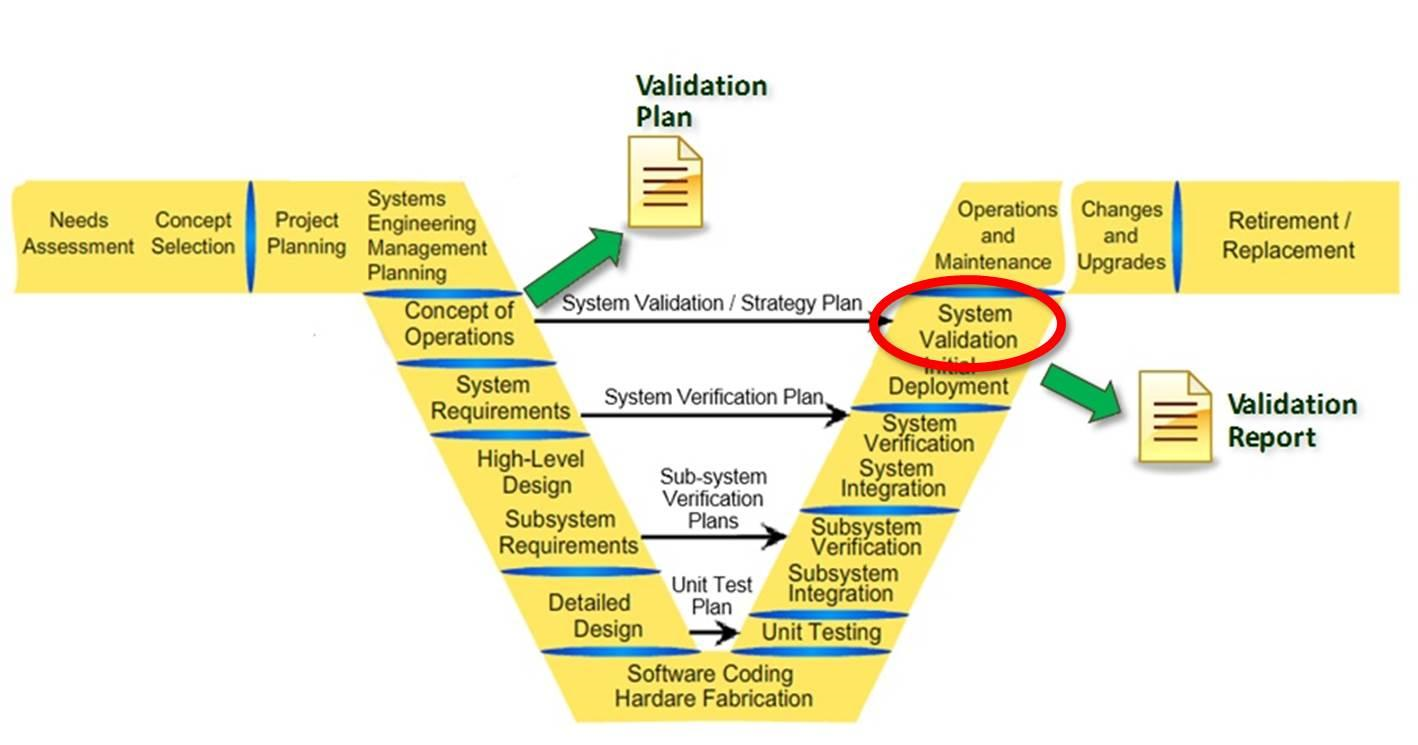
\includegraphics[scale=0.36]{figures/v_diagram_-_validation_plan2.png}
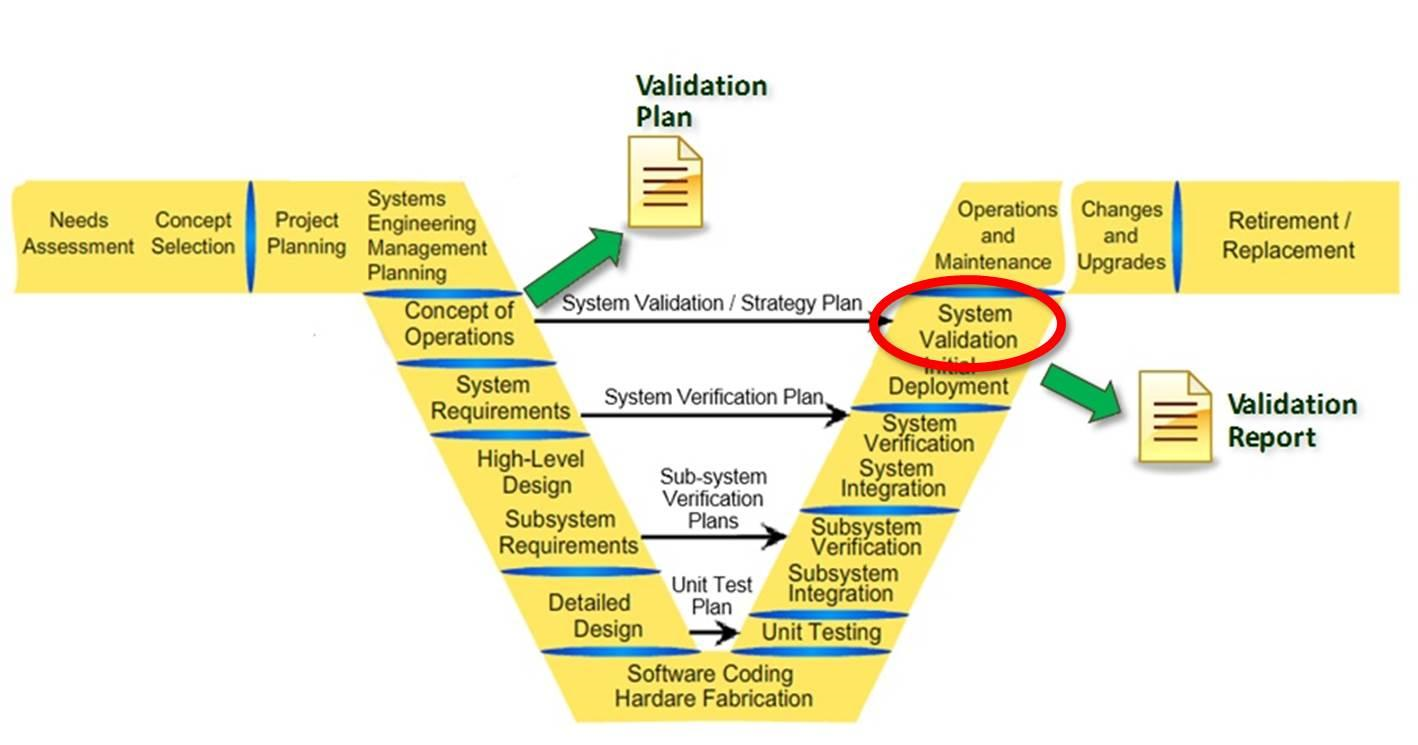
\includegraphics[scale=0.52]{figures/v_diagram_-_validation_plan2.png}
\end{center}
\caption{The V-Model of software development}
\label{fig:v-model}
\end{figure}

\pagebreak

If you bisect vertically the V-Model, you will notice that \underline{each requirement} -- or implementation -- on the left-hand side is \emph{supported} by a verification or validation step on the right-hand side.  This ensures that the scope is bounded and provides complete coverage\footnote{Coverage ensures all aspects of the codebase are verified and asserted via test(s).}.  For every step \underline{documentation is critical} to both \emph{specify} the requirements, and then to subsequently \emph{validate} against those requirements.

%all the steps throughout the development .  Types might at times seem burdensome, but if viewed correctly can provide insight in how to naturally create or evolve the construction of APIs. \\

%Below is 

\section{Testing Under Changing Environments Via System Testing}

There will be times where \emph{Integration Testing} is not enough.  This is where \index{system testing}\emph{System Testing}\footnote{Ashfaque Ahmed and Bhanu Prasad. 2016. \emph{Foundations of Software Engineering.} Auerbach Publications, Boston, MA, USA.} comes in.  Here we take the software product as a \emph{black box} --  as opposed to in Integration Testing -- and test it under different environments without touching the code-base.  One of the best ways to ensure that the software product will operate as defined by the \emph{requirements} is to run \emph{end-to-end scenarios} with validation.  This requires one to have a list of \emph{functional specifications} that the software product must perform, and to create one or more workflows where these will be pipelined together to generate this type of \index{functional testing}\emph{Functional Testing}\footnote{Functional Testing validates the software design based on the requirement specifications, by running tests to check that the software's features match the functional specifications.}.  \\

For BMI these are defined as follows: \\

\begin{itemize}
\item[\code{pro }$\blacktriangleright$\hspace{-12mm}] \hspace{10mm}\emph{Provisions a node.}
\item[\code{dpro }$\blacktriangleright$\hspace{-12mm}] \hspace{10mm}\emph{Deprovisions a node.}
\item[\code{snap }$\blacktriangleright$\hspace{-12mm}] \hspace{10mm}\emph{Takes a snapshot of a node.}
\item[\code{ls }$\blacktriangleright$\hspace{-12mm}] \hspace{10mm}\emph{Lists store images.}
\item[\code{import }$\blacktriangleright$\hspace{-12mm}] \hspace{10mm}\emph{Importing images or snapshots into BMI for provisioining.}
\item[\code{db }$\blacktriangleright$\hspace{-12mm}] \hspace{10mm}\emph{Database commands that about imported images or snapshots.} \\
\end{itemize}

By then integrating these into an end-to-end workflow, one can perform all these and ensure that the basic requirements are satisfied.  An example of a possible end-to-end workflow is described in Figure \ref{fig:end_to_end_workflow}. %as follows:

\begin{figure}[!h] % Example of including images
\vspace{10mm}
\label{fig:bmi-workflow-end-to-end}
\begin{center}
%\includegraphics[width=0.5\linewidth]{#1}
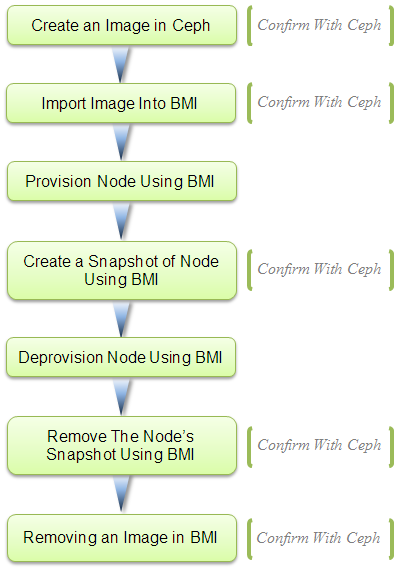
\includegraphics[scale=0.7]{figures/bmi-workflow-with-image-cleanup-v2.png}
\end{center}
\caption{An example of an end-to-end workflow}
\label{fig:end_to_end_workflow}
\end{figure}

%\section{Building a System Testing Framework via The Scientific Method}
\section{Behavior-Driven Development: A Scientific-Method Approach to Testing}

The \index{scientific method}\emph{Scientific Method} is an unbiased approach to discovering what the facts truly about a system by progressing using \emph{systematic doubt}\footnote{Morris Raphael Cohen and Ernest Nagel. 1934. \emph{An Introduction to Logic And Scientific Method.} Harcourt, Brace and World, New York, NY, USA.} to ensure adequate evidence support each problem being solved.  The facts are not gathered unless there is a problem being defined upon which relevant facts are required to prove or disprove inquiries (\emph{hypotheses}) about the problem. \\




\index{Behavior-Driven Development (BDD)}Behavior-Driven Development (BDD) is defined through a live document implemented using the Gherkin language\footnote{\link{https://github.com/cucumber/cucumber/wiki/Gherkin}}, which utilizes \emph{Given-When-Then} control-flow syntax defined as follows: \\

\begin{itemize}
\item[\index{BDD (Given)}\code{Given }$\blacktriangleright$\hspace{-12mm}] \hspace{10mm}\emph{Defines a given state.}
\item[\index{BDD (When)}\code{When }$\blacktriangleright$\hspace{-12mm}] \hspace{10mm}\emph{Defines a given action performed under the given state.}
\item[\index{BDD (Then)}\code{Then }$\blacktriangleright$\hspace{-12mm}] \hspace{10mm}\emph{Defines the expected outcome after the action is performed.} \\
\end{itemize}

By building a \emph{scenario} through combining these into premises using the \emph{Given}- and \emph{When}-initiated statements, we are able to discover if our system is validated at each step and confirm the \emph{Then} conclusion statement(s).  Thus we are hypothesis-driven through a BDD-model of our system to ensure it matches our expected \emph{operational semantics}\footnote{\link{https://en.wikipedia.org/wiki/Operational_semantics}}. \\

%\pagebreak

An example of such an end-to-end scenario for BMI is illustrated in Figure \ref{fig:chp1_bdd-bmi-end-to-end-template}, where each line is a step that references an implemented function. \\

The \index{end-to-end scenario}end-to-end scenario is a \emph{model} used as a set of \emph{rules of inference} guided by an ordered collection of \index{premises}\emph{premises} -- which are assumed to be \emph{true} -- and \index{conclusions}conclude that \emph{all} the steps are \emph{truth preserving}:

\begin{center}
$$Premises \implies Conclusions$$
\end{center}

\pagebreak

\begin{figure}[!h] % Example of including images
%\label{fig:ceph-imported-cloned-image}
\begin{center}
%\includegraphics[width=0.5\linewidth]{#1}
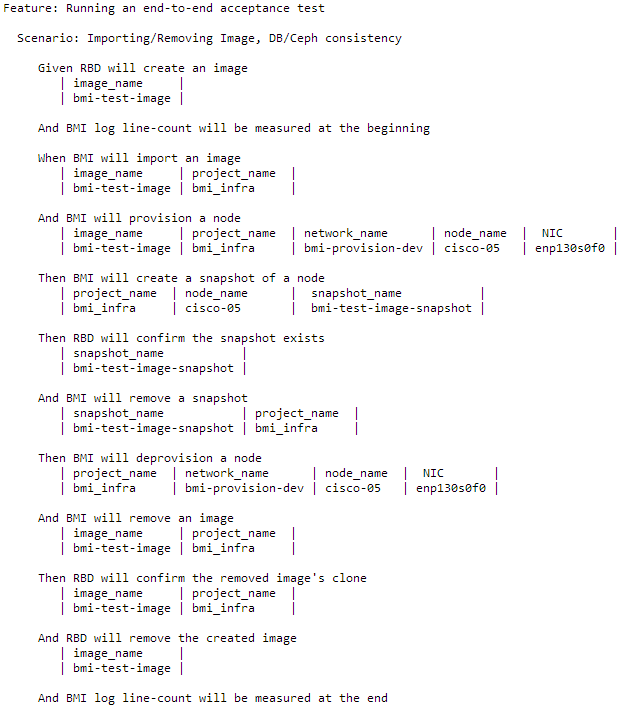
\includegraphics[scale=1]{figures/end-to-end-bdd-template.png}
\end{center}
\caption{The BMI End-to-End Behavior-Driven Deployment Test, with tables of parameters to test with}
%\label{fig:example_figure}
\label{fig:chp1_bdd-bmi-end-to-end-template}
\end{figure}





For example, in Figure \ref{fig:chp1_bdd-bmi-function-definition} the creation of a RADOS block device (RBD\footnote{Ceph Storage provides the ability for its (bootable) images to be mountable remotely using a RADOS block device.  For more information please proceed to the following web location: \\  \link{https://docs.openstack.org/mitaka/config-reference/block-storage/drivers/ceph-rbd-volume-driver.html}}) mountable image at the start is defined through the \code{rbd\_create\_image()} function, where it is decorated by the sentence referenced in the live-document. \\

\text{}\vspace{10mm}

\pagebreak

%
\begin{figure}[!h] % Example of including images
%\label{fig:ceph-imported-cloned-image}
\begin{center}
%\includegraphics[width=0.5\linewidth]{#1}
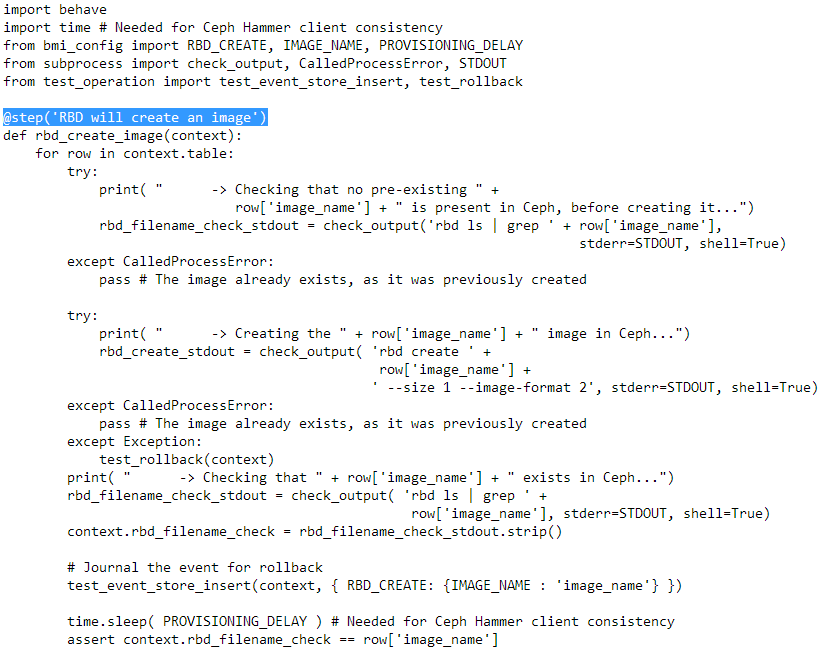
\includegraphics[scale=1]{figures/bmi-bdd-step-definition-v3.png}
\end{center}
\caption{The definition of the RBD creation step, where the decoration highlights the sentence referenced in the end-to-end deployment test}
%\label{fig:example_figure}
\label{fig:chp1_bdd-bmi-function-definition}
\end{figure}

\text{}\vspace{10mm}

In the next chapter, you will learn how to configure and run an acceptance test.
\part{Getting Started With The User Acceptance Testing Framework}
\labelPart{Using_BMI}
% SVN info for this file
\svnidlong
{$HeadURL$}
{$LastChangedDate$}
{$LastChangedRevision$}
{$LastChangedBy$}

\chapter{Working With BMI}
\labelChapter{Chapter_2}

\begin{introduction}
  This chapter will guide through the steps of working with BMI.
\end{introduction}

\section{Core Commands in BMI}

We will explore the following six commands in BMI: \\

\begin{itemize}
\item[\index{bmi pro}\code{pro }$\blacktriangleright$\hspace{-12mm}] \hspace{10mm}\emph{Provisions a node.}
\item[\index{bmi dpro}\code{dpro }$\blacktriangleright$\hspace{-12mm}] \hspace{10mm}\emph{Deprovisions a node.}
\item[\index{bmi snap}\code{snap }$\blacktriangleright$\hspace{-12mm}] \hspace{10mm}\emph{Takes a snapshot of a node.}
\item[\index{bmi ls}\code{ls }$\blacktriangleright$\hspace{-12mm}] \hspace{10mm}\emph{Lists store images.}
\item[\index{bmi ls}\code{import }$\blacktriangleright$\hspace{-12mm}] \hspace{10mm}\emph{Importing images or snapshots into BMI for provisioining.}
\item[\index{bmi db}\code{db }$\blacktriangleright$\hspace{-12mm}] \hspace{10mm}\emph{Database commands that about imported images or snapshots.} \\
\end{itemize}

Using these commands we will run through the end-to-end workflow shown in Figure \ref{fig:bmi-workflow-end-to-end}. 


%\pagebreak

\begin{figure}[!h] % Example of including images
\vspace{10mm}
\label{fig:bmi-workflow-end-to-end}
\begin{center}
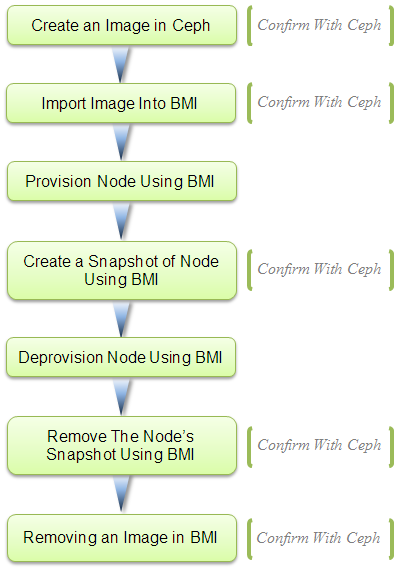
\includegraphics[scale=1.2]{figures/bmi-workflow-with-image-cleanup-v2.png}
\end{center}
\caption{HIL and BMI Ecosystem}
%\label{fig:example_figure}
\end{figure}


\section{Creating a Mock HIL and BMI Ecosystem}


In order to better learn how to use BMI, we will need to setup the a Ceph storage location, HIL and BMI instance.  The first step is to ensure that one has either a RedHat Enterprise Linux or Ubuntu instance with at least 5 GB of available storage with \code{sudo} access.  This can be performed via a virtual machine (VM).  Once that is created and you booted into the machine, you will need to \code{git-clone} the setup scripts, via the steps provided on the following page.

\pagebreak

\code{
\text{}\vspace{-10mm} \\
\text{}\hspace{6mm} git clone https://github.com/CCI-MOC/ims.git \\
\text{}\hspace{6mm} cd ims \\
\text{}\hspace{6mm} git fetch origin pull/60/head:pr-60 \\
\text{}\hspace{6mm} git checkout pr-60 \\
}

This will ensure that you have the proper install scripts and codebase to install Ceph, HIL and BMI.

\pagebreak

\subsection{Installing Ceph, HIL and BMI}

First it is important to prepare the environment for installation.  It is recommended you use either CentOS or Ubuntu (preferred) for your installation.  Each of these might require one to perform these commands: \\

\underline{\emph{For Ubuntu}} 

\code{
\text{} \\
\text{}\hspace{6mm} sudo add-apt-repository -y ppa:fkrull/deadsnakes \\
\text{}\hspace{6mm} sudo apt-get -y update \\
\text{}\hspace{6mm} sudo apt-get -y install python2.7 \\
\text{}\hspace{6mm} sudo ln -s /usr/bin/python2.7 /usr/bin/python \\
}

\underline{\emph{For CentOS}} 

\code{
\text{} \\
\text{}\hspace{6mm} sudo yum -y install git \\
}

Next you will need to prepare the Ceph configuration file by going to the install directory, as follows:

%In order to install type the following at the Bash prompt: 


\code{
\text{} \\
\text{}\hspace{6mm} cd scripts/install/ \\
%\text{}\hspace{6mm} ./install.sh \\
}

And subsequently running the following Ceph configuration script:


\code{
\text{} \\
\text{}\hspace{6mm} \small\#!/bin/bash \\
\text{}\hspace{6mm} if [ ! -z  "`sudo ls /etc/ | grep redhat-release`" ]; then \\
\text{}\hspace{12mm}   cp /etc/hostname . \\
\text{}\hspace{12mm}   cat /etc/hostname | cut -f1 -d'.' > hostname \\
\text{}\hspace{12mm}   sudo cp hostname /etc \\
\text{}\hspace{6mm} fi \\
\text{}\hspace{6mm} if [ ! -z "`ifconfig | grep inet | head -n1 | grep :`" ]; then \\
\text{}\hspace{12mm}   IP\_ADDRESS=`ifconfig | grep inet | head -n1 | cut -f2 -d':' | cut -f1 -d' '` \\
\text{}\hspace{6mm} else \\
\text{}\hspace{12mm}   IP\_ADDRESS=`ifconfig | grep inet | head -n1 | cut -f2 -d'i' | cut -f2 -d' '` \\
\text{}\hspace{6mm} fi \\
\text{}\hspace{6mm} echo -e "public\_network = \$IP\_ADDRESS/24\textbackslash{}nosd pool default size = 2\textbackslash{}nosd crush chooseleaf type = 0" >{}> ceph.conf \\
}

At this point you can initiate the installation process as follows:

\code{
\text{} \\
%\text{}\hspace{6mm} cd scripts/install/ \\
\text{}\hspace{6mm} ./install.sh \\
}

\pagebreak

After the installation first check that \index{Ceph}Ceph is operational:

\code{
\text{} \\
\text{}\hspace{6mm} ceph -s \\
}

You should see the following, which should be indicated by \code{HEALTH\_OK} under the \emph{health} attribute:

\code{
\text{} \\
\text{}\hspace{6mm} cluster 2469e0b1-9269-434a-8dc5-047c863f70e0 \\
\text{}\hspace{6mm} health HEALTH\_OK \\
\text{}\hspace{6mm} monmap e1: 1 mons at {pgrosu-pr-60=192.168.1.14:6789/0} \\
\text{}\hspace{12mm} election epoch 3, quorum 0 pgrosu-pr-60 \\
\text{}\hspace{6mm} osdmap e31: 3 osds: 3 up, 3 in \\
\text{}\hspace{12mm} flags sortbitwise,require\_jewel\_osds \\
\text{}\hspace{6mm} pgmap v87: 112 pgs, 7 pools, 19066 kB data, 184 objects \\
\text{}\hspace{12mm} 140 MB used, 14466 MB / 14606 MB avail \\
\text{}\hspace{22mm} 112 active+clean \\
}

Next check the \index{Ceph}Ceph version via the following command: 

\code{
\text{} \\
\text{}\hspace{6mm}  ceph --version \\
}

You should see the following output: 

\code{
\text{} \\
\text{}\hspace{6mm} ceph version 10.2.7 (50e863e0f4bc8f4b9e31156de690d765af245185) \\
}

Next check the \index{ceph-deploy}\code{ceph-deploy} version via the following command: 

\code{
\text{} \\
\text{}\hspace{6mm} ceph-deploy --version \\
}

You should see the following output: 

\code{
\text{} \\
\text{}\hspace{6mm} 1.5.38 \\
}

Next check that \index{RBD}RBD is operational via the following command: 

\code{\text{} \\
\text{}\hspace{6mm} rbd ls \\
}

\pagebreak

You should see the following listed images: 

\code{
\text{} \\
\text{}\hspace{6mm} 112233445566778899img1 \\
\text{}\hspace{6mm} cirros-0.3.0-x86\_64-disk.img \\
}

%\pagebreak

Next you will need to set the HIL \emph{username} and \emph{password} that is in the \code{bmi\_userrc.sh} file, by typing the following command:

\code{
\text{} \\
\text{}\hspace{6mm} source bmi\_userrc.sh \\
}

That file just contains the following two entries: 

%\pagebreak 

\code{
\text{} \\
\text{}\hspace{6mm} export HAAS\_USERNAME=haas \\
\text{}\hspace{6mm} export HAAS\_PASSWORD=secret \\
}

Next we can enter the BMI virtual environment via the following two commands: 

\code{
\text{} \\
\text{}\hspace{6mm} cd $\sim$/ims/ \\
\text{}\hspace{6mm} source .bmi\_venv/bin/activate \\
}

You will know that you are in the virtual environment if you see the prompt being prefixed by \code{(.bmi\_venv)} displayed as follows: 

\code{
\text{} \\
\text{}\hspace{6mm} (.bmi\_venv) ubuntu@pgrosu-pr-60:$\sim$/ims\$ \\
} 

The Einstein and Picasso servers are already running, which you can verify by the following command: \\

\code{
\text{} \\
\text{}\hspace{6mm} ps -Af | grep server | grep -iv color \\
}

You should see \emph{one} Picasso server process, and \emph{three} Einstein server processes: 

\code{
\text{} \\
\text{}\hspace{6mm} ubuntu   22670     1  0 15:01 pts/0    00:00:00 python scripts/picasso\_server \\
\text{}\hspace{6mm} ubuntu   22669     1  0 15:01 pts/0    00:00:00 python scripts/einstein\_server \\
\text{}\hspace{6mm} ubuntu   22680 22669  0 15:01 pts/0    00:00:00 python scripts/einstein\_server \\
\text{}\hspace{6mm} ubuntu   22681 22669  0 15:01 pts/0    00:00:00 python scripts/einstein\_server \\
}

\begin{tcblisting}{%
    warning,
    listing only, 
    title=Configuring BMI, fonttitle=\bfseries
  } 
To ensure that the BMI debug output does not show up during the BMI 
workflow, please type the following commands:

cat /etc/bmi/bmiconfig.cfg | sed -e 's/true/false/g' > bmiconfig.cfg 
mv bmiconfig.cfg /etc/bmi/bmiconfig.cfg 

\end{tcblisting}


\subsection{The HIL Configuration}

Remember that we need the ports on the switch to be pre-configured with the project (VLAN network isolation) for the NIC (node) we will provision.  That has been performed via the \code{install\_hil.sh} scirpt, which can be accessed here: \\

\scriptsize\link{https://github.com/sirushtim/ims/blob/327acf2db0094e331ca0d9b734b8b99a64f722a4/scripts/install/install_hil.sh}

\normalsize This script will setup HIL to create the \emph{network}, \emph{project}, \emph{node} and register them properly with the \emph{switch} using the following commands:

\code{
\text{} \\
\text{}\hspace{6mm} \# Create Haas projects \\
\text{}\hspace{6mm} haas project\_create bmi\_infra \\
\text{} \\
\text{}\hspace{6mm} \#\#\# Setup HaaS mock node \\
\text{}\hspace{6mm} haas node\_register bmi\_node mock moch-hostname mock-username mock-password \\
\text{}\hspace{6mm} haas project\_connect\_node bmi\_infra bmi\_node \\
\text{} \\
%\text{}\hspace{6mm} \#\#\# Tell HaaS the mac address of the node \\
\text{}\hspace{6mm} \#\#\# Tell HaaS the MAC address of the NIC \\
\text{}\hspace{6mm} haas node\_register\_nic bmi\_node bmi\_port "00:00:00:00:00:00" \\
\text{} \\
\text{}\hspace{6mm} \#\#\# Setup HaaS switch \\
\text{}\hspace{6mm} haas switch\_register bmi\_switch mock moch-hostname mock-username mock-password \\
\text{}\hspace{6mm} haas port\_register bmi\_switch bmi\_port \\
\text{}\hspace{6mm} haas port\_connect\_nic bmi\_switch bmi\_port bmi\_node bmi\_port \\
\text{} \\
\text{}\hspace{6mm} \#\#\# Setup HaaS network \\
\text{}\hspace{6mm} haas network\_create\_simple bmi\_network bmi\_infra \\
}

The above HIL code defines the following variables, which are required for BMI: \\

\begin{itemize}
\item[\emph{Project }$\blacktriangleright$\hspace{-21mm}] \hspace{19mm} \code{bmi\_infra} \\
\item[\emph{Node }$\blacktriangleright$\hspace{-21mm}] \hspace{19mm} \code{bmi\_node} \\ %\item[Project] bmi-test-image 
\item[\emph{Network }$\blacktriangleright$\hspace{-21mm}] \hspace{19mm} \code{bmi\_network} \\
\item[\emph{NIC }$\blacktriangleright$\hspace{-21mm}] \hspace{19mm} \code{bmi\_port} \\
\end{itemize}

Now that the environment is properly set up, you can use BMI to step through the workflow.

\section{Using BMI}

\subsection{Creating a new image}

First we need to create a new image using \code{rbd} in Ceph for BMI to use: \\

% rbd create bmi-test-image --size 1 --image-format 2
\index{rbd create}\code{rbd create bmi-test-image -{}-size 1 -{}-image-format 2} \\

To ensure the new image exists run \code{rbd ls} and you should see the following: 

\code{
\text{} \\
\text{}\hspace{6mm} 112233445566778899img1 \\
\text{}\hspace{6mm} bmi-test-image \\
\text{}\hspace{6mm} cirros-0.3.0-x86\_64-disk.img 
}

\subsection{Import the new image into BMI}

To \index{import}import the image into BMI type the following command: 

\code{
\text{} \\
\text{}\hspace{6mm} \index{bmi import}bmi import bmi\_infra bmi-test-image \\
}

To ensure the new image imported run \index{bmi db ls}\code{bmi db ls} and you should see the following: \\


\begin{figure}[!h] % Example of including images
\label{fig:bmi-workflow}
\begin{center}
%\includegraphics[width=0.5\linewidth]{#1}
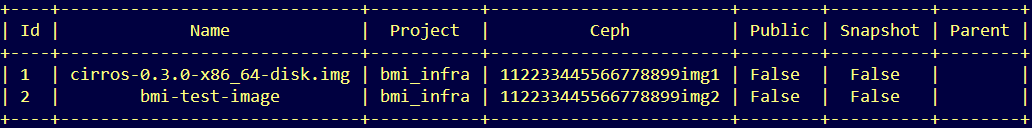
\includegraphics[scale=0.7]{figures/bmi-import-db-ls.png}
\end{center}
\caption{The output of running: \code{bmi db ls}}
%\label{fig:example_figure}
\end{figure}

The same thing can be viewed through the following command: \\

\code{
\text{} \\
\text{}\hspace{6mm} \index{bmi ls}bmi ls bmi\_infra \\
}

This will result in the following output:

\begin{figure}[!h] % Example of including images
\label{fig:bmi-workflow}
\begin{center}
%\includegraphics[width=0.5\linewidth]{#1}
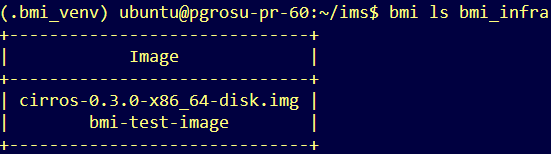
\includegraphics[scale=0.7]{figures/bmi-ls.png}
\end{center}
\caption{The output of running: \code{bmi ls}}
\end{figure}


Notice in Figure \ref{fig:ceph-imported-cloned-image} how in Ceph there now is a cloned image created with the name \code{112233445566778899img2}, since the golden image named \code{bmi-test-image} must be preserved.



\begin{figure}[!h] % Example of including images
\begin{center}
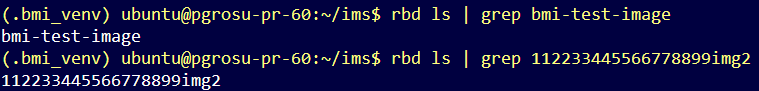
\includegraphics[scale=0.7]{figures/rbd-ls-bmi-test-image.png}
\end{center}
\caption{The seeing the images in Ceph}
%\label{fig:example_figure}
\label{fig:ceph-imported-cloned-image}
\end{figure}


\pagebreak

\subsection{Provisioning a Node Using BMI}

To \index{provision}provision a node in BMI, type the following command: 


\code{
\text{} \\
\text{}\hspace{6mm} \index{bmi pro}bmi pro bmi\_infra bmi\_node bmi-test-image bmi\_network bmi\_port \\
}

If the above processes successfully, you should see \code{Success} printed on your terminal screen, as follows: \\

\begin{figure}[!h] % Example of including images
\label{fig:bmi-workflow}
\begin{center}
%\includegraphics[width=0.5\linewidth]{#1}
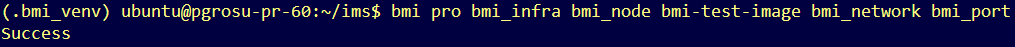
\includegraphics[scale=0.7]{figures/bmi-provisioning.png}
\end{center}
\caption{The output of running BMI provisioning command}
%\label{fig:example_figure}
\end{figure}

To see the new snapshot in BMI, run \index{bmi db ls}\code{bmi db ls} and you should see the following: \\

\begin{figure}[!h] % Example of including images
\label{fig:bmi-workflow}
\begin{center}
%\includegraphics[width=0.5\linewidth]{#1}
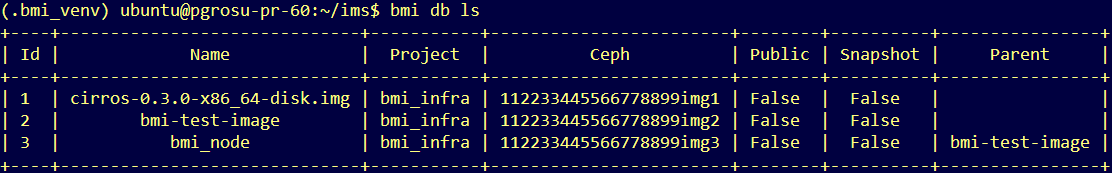
\includegraphics[scale=0.7]{figures/bmi-provisioning-db-ls.png}
\end{center}
\caption{Listing the newly provisioning in BMI}
%\label{fig:example_figure}
\end{figure}

%\pagebreak

Notice how the name is the node name itself (\code{bmi\_node}) who's parent is \code{bmi-test-image} is listed, with the \code{Parent} column set to \code{bmi-test-image}.   \\


\subsection{Creating a Snapshot Using BMI}

Snapshots provide the ability to get an instance of a state of an image at a point-in-time.  These are just a read-only copy, which would require to be cloned and flattened\footnote{Flattening an image makes it independent from the parent snapshot by copying the data to the child image.} in order to be writeable.   Snapshots in fact are central to protecting a golden image on Ceph, so that the original is preserved. \\

\pagebreak

To create a \index{snapshot}snapshot of a node in BMI, first make sure that the \underline{node is powered off}, and then type the following command: 

\code{
\text{} \\
\text{}\hspace{6mm} \index{bmi snap create}bmi snap create bmi\_infra bmi\_node bmi-test-image-snapshot \\
}

%\pagebreak

If the above processes successfully, you should see \code{Success} printed on your terminal screen, as follows: \\


\begin{figure}[!h] % Example of including images
\label{fig:bmi-workflow}
\begin{center}
%\includegraphics[width=0.5\linewidth]{#1}
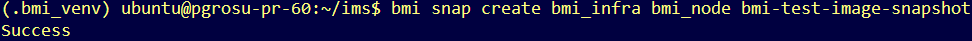
\includegraphics[scale=0.7]{figures/bmi-snapshot-create.png}
\end{center}
\caption{The output of creating a snapshot using BMI}
%\label{fig:example_figure}
\end{figure}



To see the new snapshot in BMI, run \index{bmi db ls}\code{bmi db ls} and you should see the following: \\

%\pagebreak

\begin{figure}[!h] % Example of including images
\label{fig:bmi-workflow}
\begin{center}
%\includegraphics[width=0.5\linewidth]{#1}
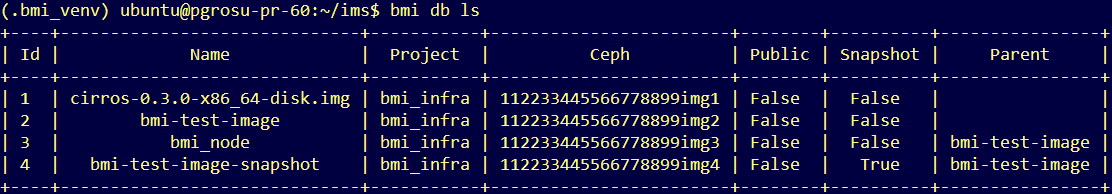
\includegraphics[scale=0.7]{figures/bmi-snapshot-db-ls.png}
\end{center}
\caption{Listing the newly created snapshot in BMI}
%\label{fig:example_figure}
\end{figure}


Notice how the \code{Snapshot} column is now set to \code{True}, with the \code{Parent} column set to \code{bmi-test-image}. \\  

%\pagebreak 

To see what is stored in Ceph, below is the output of running \code{rbd ls -l}: \\

\begin{figure}[!h] % Example of including images
\label{fig:bmi-workflow}
\begin{center}
%\includegraphics[width=0.5\linewidth]{#1}
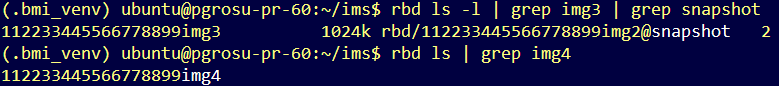
\includegraphics[scale=0.7]{figures/rbd-ls-snapshot.png}
\end{center}
\caption{The stored files in Ceph.}
%\label{fig:example_figure}
\end{figure}



\subsection{Deprovisioning a Node Using BMI}

To \index{deprovision}deprovision a node in BMI, type the following command: 

% bmi import bmi_infra bmi-test-image

\code{
\text{} \\
\text{}\hspace{6mm} \index{bmi dpro}bmi dpro bmi\_infra bmi\_node bmi\_network bmi\_port \\
}

If the above processes successfully, you should see \code{Success} printed on your terminal screen, as follows: \\


\begin{figure}[!h] % Example of including images
\label{fig:bmi-workflow}
\begin{center}
%\includegraphics[width=0.5\linewidth]{#1}
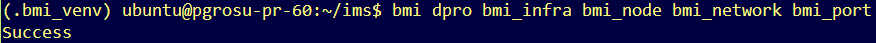
\includegraphics[scale=0.7]{figures/bmi-deprovisioning.png}
\end{center}
\caption{The output of running BMI deprovisioning command}
%\label{fig:example_figure}
\end{figure}

%\pagebreak

To see how BMI is updated, run \index{bmi db ls}\code{bmi db ls} and you should see the following: \\

\begin{figure}[!h] % Example of including images
\label{fig:bmi-workflow}
\begin{center}
%\includegraphics[width=0.5\linewidth]{#1}
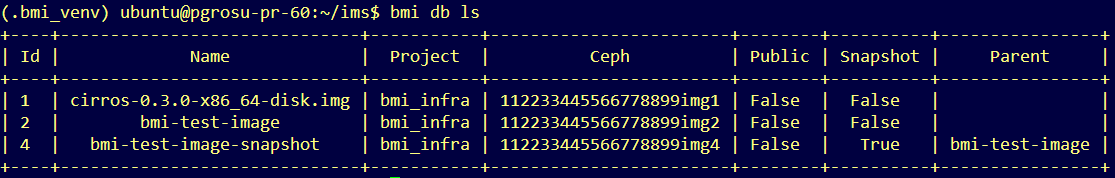
\includegraphics[scale=0.7]{figures/bmi-deprovisioning-db-ls.png}
\end{center}
\caption{Listing the newly created snapshot in BMI}
%\label{fig:example_figure}
\end{figure}




\subsection{Removing a Snapshot Using BMI}

To \index{remove a snapshot}remove a snapshot of a node in BMI, type the following command: 

\code{
\text{} \\
\text{}\hspace{6mm} \index{bmi snap rm}bmi snap rm bmi\_infra bmi-test-image-snapshot \\
}

%\pagebreak

If the above processes successfully, you should see \code{Success} printed on your terminal screen, as follows: \\

%\pagebreak


\begin{figure}[!h] % Example of including images
\label{fig:bmi-workflow}
\begin{center}
%\includegraphics[width=0.5\linewidth]{#1}
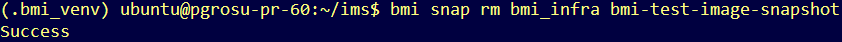
\includegraphics[scale=0.7]{figures/bmi-snapshot-remove.png}
\end{center}
\caption{The output of removing a snapshot using BMI}
%\label{fig:example_figure}
\end{figure}

To see that the \index{snapshot}snapshot was removed in BMI, run \index{bmi db ls}\code{bmi db ls} and you should see the following: \\

\begin{figure}[!h] % Example of including images
\label{fig:bmi-workflow}
\begin{center}
%\includegraphics[width=0.5\linewidth]{#1}
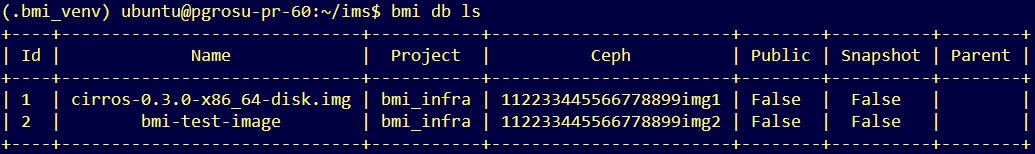
\includegraphics[scale=0.7]{figures/bmi-snapshot-remove-db-ls.png}
\end{center}
\caption{Showing that the snapshot was removed in BMI}
%\label{fig:example_figure}
\end{figure}

%\pagebreak 

To see that the snapshot does not exist in Ceph, below is the output of running \\
\code{rbd ls -l}: \\

\begin{figure}[!h] % Example of including images
\label{fig:bmi-workflow}
\begin{center}
%\includegraphics[width=0.5\linewidth]{#1}
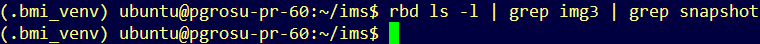
\includegraphics[scale=0.7]{figures/rbd-ls-snapshot-removed.png}
\end{center}
\caption{Showing that the snapshot does not exist in Ceph}
%\label{fig:example_figure}
\end{figure}



\subsection{Removing an Image Using BMI}

To \index{remove an image}remove an image in BMI, type the following command: 

\code{
\text{} \\
\text{}\hspace{6mm} \index{bmi rm}bmi rm bmi\_infra bmi-test-image \\
}

%\pagebreak

If the above processes successfully, you should see \code{Success} printed on your terminal screen, as follows: \\

%\pagebreak


\begin{figure}[!h] % Example of including images
\label{fig:bmi-workflow}
\begin{center}
%\includegraphics[width=0.5\linewidth]{#1}
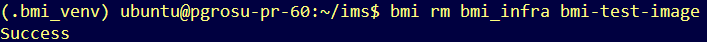
\includegraphics[scale=0.7]{figures/bmi-rm-db-ls.png}
\end{center}
\caption{The output of removing an image using BMI}
%\label{fig:example_figure}
\end{figure}

To see that the image was removed in BMI, run \index{bmi db ls}\code{bmi db ls} and you should see the following: \\

\begin{figure}[!h] % Example of including images
\label{fig:bmi-workflow}
\begin{center}
%\includegraphics[width=0.5\linewidth]{#1}
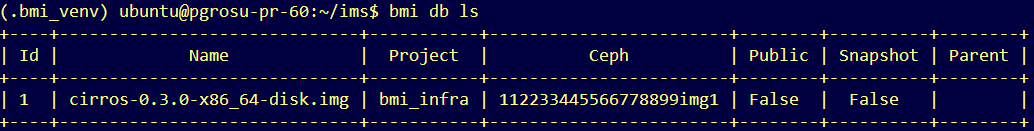
\includegraphics[scale=0.7]{figures/bmi-image-remove-db-ls.png}
\end{center}
\caption{Showing that the image was removed in BMI}
%\label{fig:example_figure}
\end{figure}


%\pagebreak 

To remove the image from Ceph, just type the following command:

\code{
\text{} \\
\text{}\hspace{6mm} \index{rbd rm}rbd rm bmi-test-image \\
}
 
You should now see that the image does not exist in Ceph, below is the output of running \\
\index{rbd ls}\code{rbd ls}: \\

\begin{figure}[!h] % Example of including images
\label{fig:bmi-workflow}
\begin{center}
%\includegraphics[width=0.5\linewidth]{#1}
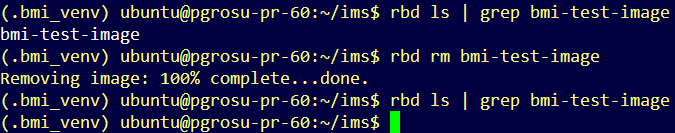
\includegraphics[scale=0.7]{figures/rbd-rm-bmi-test-image.png}
\end{center}
\caption{Showing that the image does not exist in Ceph}
%\label{fig:example_figure}
\end{figure}

\section{Existing the Virtual Environment}

To exit \index{virtualenv}\code{virtualenv}, type the following command: 

\code{
\text{} \\
\text{}\hspace{6mm} deactivate \\
}

%\pagebreak

Your terminal prompt should change to the following after typing the command: \\

\begin{figure}[!h] % Example of including images
\label{fig:bmi-workflow}
\begin{center}
%\includegraphics[width=0.5\linewidth]{#1}
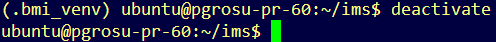
\includegraphics[scale=0.7]{figures/virtualenv-exit.png}
\end{center}
\caption{Existing the Virtual Environment \code{virtualenv}}
%\label{fig:example_figure}
\end{figure}


This completes the end-to-end training for learning how to use the most common BMI commands.


%% SVN info for this file
\svnidlong
{$HeadURL$}
{$LastChangedDate$}
{$LastChangedRevision$}
{$LastChangedBy$}

\chapter{BMI Internals}
\labelChapter{Chapter_3}

\begin{introduction}
  This chapter will describe some of the internals of how BMI works.
\end{introduction}

% to create and index select MakeIndex -> Run arrow, and then switch to pdfLaTeX and Run Arrow

\section{The Clone-Snapshot Workflow}

Central to the \index{BMI methodology}BMI methodology - especially with a Ceph networked-storage cluster, servicing images via a \index{RADOS Block Device (RBD)}\emph{RADOS Block Device (RBD)} - is the \index{Clone-Snapshot workflow}\emph{Clone-Snapshot} workflow: \\

\begin{figure}[!h] % Example of including images
\label{fig:bmi-workflow-import}
\begin{center}
%\includegraphics[width=0.5\linewidth]{#1}
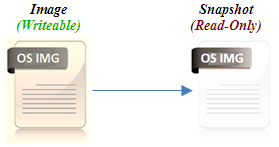
\includegraphics[scale=1]{figures/ceph-clone-snapshot.png}
\end{center}
\caption{The Clone-Snapshot Workflow}
%\label{fig:example_figure}
\end{figure}


Images are files used to iPXE boot from, which can also be written to.  Images \underline{\emph{cannot}} be cloned, though if one creates a snapshot - which is a point-in-time, read-only copy of an image that preserves its state - one can \index{clone}clone that \index{snapshot}snapshot to create a new child image.  These child images are now connected to the parent snapshot, but one can \index{flatten}\emph{flatten} them in order to copy over any dependent data to sever this connection, and thus make them independent. Therefore in order to ensure provenance, and also be able to extend the BMI workflow through new customized images, one always will create a snapshot after creating or cloning/flattening a new image.  By guaranteeing that all images will have a snapshot, one will always be able to connect to any image's snapshot to inherit and extend its state cloning.  All snapshots associated with images that are created through BMI are named \code{snapshot}. \\


The general overview connection between Ceph, RADOS, snapshots and images is illustrated in Figure \ref{fig:ceph_rados_snapshot_clone}\footnote{\link{https://www.packtpub.com/books/content/working-ceph-block-device}}. \\


\begin{figure}[!h] % Example of including images
\label{fig:bmi-workflow-import}
\begin{center}
%\includegraphics[width=0.5\linewidth]{#1}
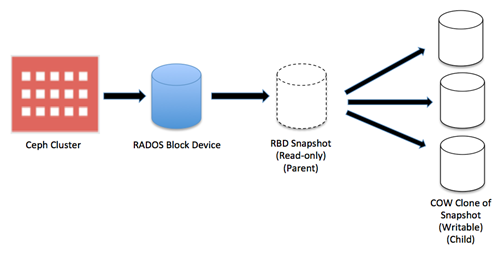
\includegraphics[scale=1]{figures/ceph-rados-snapshot-clone.png}
\end{center}
\caption{A Ceph cluster servicing a RADOS block device providing access to snapshots and images}
\label{fig:ceph_rados_snapshot_clone}
\end{figure}


\section{Importing an Image}

The concept behind importing an image into BMI is to create a duplicate of the image - considered the \index{Golden Image}\emph{Golden Image} in Ceph - so that we have a golden image from BMI's perspective to extend from.  The database column in BMI called \code{Ceph} contains the images associated with that instance of BMI, that are stored in Ceph.  Now any subsequent operation on a row in the \code{Name} column from the BMI database --- such as \emph{provisioning} or \emph{snapshotting} --- will actually clone the image's snapshot indicated in the \code{Ceph} column for that respective row of that name, and then create a snapshot as well. \\

The one difference when importing an image into BMI, is that there might not be a snapshot in the original image in Ceph.  For that reason, every time an image is imported into BMI, a snapshot is taken.  Afterwards a \index{clone-and-flatten}\emph{clone-and-flatten} operation is performed with a subsequent snapshot.  Since the flattening step makes the child image independent, BMI will remove the parent snapshot in order to save space.  In Figure \ref{fig:bmi-workflow-import}, the steps described above illustrate this workflow: \\ 


\begin{figure}[!h] % Example of including images
\label{fig:bmi-workflow-import}
\begin{center}
%\includegraphics[width=0.5\linewidth]{#1}
\includegraphics[scale=1]{figures/workflow-bmi-import-v2.png}
\end{center}
\caption{BMI Import Workflow}
%\label{fig:example_figure}
\end{figure}

\pagebreak

The steps that take place when importing and image into BMI are described in the following lines of code:

\begin{center}
\link{https://github.com/CCI-MOC/ims/blob/dev/ims/einstein/operations.py\#L431-L454}
\end{center}


\subsection{\index{Ceph image database name format}Ceph Image Name Format In The BMI Database}

One thing to mention, is that any image entry into the database under the \code{Ceph} column will be formatted using the following nomenclature: 

\begin{center}
\emph{\color{gray}PREFIX}\code{img}\emph{\color{gray}SUFFIX} 
\end{center}

The \code{PREFIX} is configured via the \code{/etc/bmi/bmiconfig.cfg} file, through the \code{uid} variable --- available under the \code{[bmi]} heading:

\code{
\text{} \\
\text{}\hspace{6mm} [bmi] \\
\text{}\hspace{6mm} uid = 5 \\
}

The \code{SUFFIX} begin with 1 and will continue to increment with every new addition to the database.  The same value will also stored under the \code{Id} column.


%\appendix
%\part{Appendices}
%\labelPart{appendices}
%% SVN info for this file
\svnidlong
{$HeadURL$}
{$LastChangedDate$}
{$LastChangedRevision$}
{$LastChangedBy$}

\chapter{Appendix}
\labelAppendix{appendix}

\begin{introduction}
  This appendix will provide a overview of the User Acceptance Testing for BMI, and for details please consult the \emph{Administrator's Guide: BMI User Acceptance Testing Framework}.
\end{introduction}

\section{User Acceptance Testing}

\lettrine[nindent=-1pt]{U}{ser Acceptance Testing} \index{User Acceptance Testing (UAT)}implementation has been added to BMI in order validate a deployment through a black-box end-to-end system test.  This performs a \index{Behavior-Driven Development (BDD)}\emph{Behavior-Driven Development} scenario using the \code{behave}\footnote{\link{http://pythonhosted.org/behave/}} Python package.  

\subsection{Behavior-Driven Development (BDD)}

Behavior-Driven Development is defined through a live-document implemented using the Gherkin language\footnote{\link{https://github.com/cucumber/cucumber/wiki/Gherkin}}, which utilizes \emph{Given-When-Then} control-flow syntax defined as follows: \\

\begin{itemize}
\item[\code{Given }$\blacktriangleright$\hspace{-12mm}] \hspace{10mm}\emph{Defines a given state.}
\item[\code{When }$\blacktriangleright$\hspace{-12mm}] \hspace{10mm}\emph{Defines a given action performed under the given state.}
\item[\code{Then }$\blacktriangleright$\hspace{-12mm}] \hspace{10mm}\emph{Defines the expected outcome after the action is performed.} \\
\end{itemize}

In Figure \ref{fig:bdd-bmi-end-to-end-template} is defined the end-to-end test performing a scenario of steps, where each line is a step that refers to a function.

\pagebreak

\begin{figure}[!h] 
%\label{fig:ceph-imported-cloned-image}
\begin{center}
%\includegraphics[width=0.5\linewidth]{#1}
\includegraphics[scale=1]{figures/end-to-end-bdd-template.png}
\end{center}
\caption{The BMI End-to-End Behavior-Driven Deployment Test, with tables of parameters to test with}
%\label{fig:example_figure}
\label{fig:bdd-bmi-end-to-end-template}
\end{figure}

For example, in Figure \ref{fig:bdd-bmi-function-definition} the creation of an RBD image at the start is defined through the \code{rbd\_create\_image()} function, where it is decorated by the sentence referenced in the live-document.

%\pagebreak

\begin{figure}[!h] 
%\label{fig:ceph-imported-cloned-image}
\begin{center}
%\includegraphics[width=0.5\linewidth]{#1}
\includegraphics[scale=1]{figures/bmi-bdd-step-definition-v3.png}
\end{center}
\caption{The definition of the RBD creation step, where the decoration highlights the sentence referenced in the end-to-end deployment test}
%\label{fig:example_figure}
\label{fig:bdd-bmi-function-definition}
\end{figure}
\text{}\vspace{10mm}
\pagebreak

\subsection{Configuring the Acceptance Tests  \\ }

\index{configuring User Acceptance Tests}Before running the acceptance tests, it is necessary to configure BMI service to test.  This is performed by the following steps:

\begin{enumerate}

\item Copy the \code{acceptance-tests} directory to the new environment. \\
\item Proceed to the \code{config/tests-uat} directory and duplicate recursively one of the configuration, as such: \\

\code{     cp -r neu-haas-dev NEW\_BMI\_SERVICE\_TO\_TEST} \\

\pagebreak

   Example: \\

\code{     cp -r neu-haas-dev prb-bu-dev} \\

\item Enter the newly created directory and update the \code{config} file accordingly.  Below is an example of one: 

\code{
\text{}\hspace{6mm}   \\
\text{}\hspace{6mm}        export BMI\_RELEASE\_NAME=moc-0.5-release \\
\text{}\hspace{6mm}   \\
\text{}\hspace{6mm}        export BMI\_PROJECT=bmi\_infra \\
\text{}\hspace{6mm}        export HIL\_NODE=cisco-05 \\
\text{}\hspace{6mm}        export HIL\_NETWORK=bmi-provision-dev \\
\text{}\hspace{6mm}        export BMI\_IMAGE\_NAME=bmi-test-image \\
\text{}\hspace{6mm}        export BMI\_SNAPSHOT\_NAME=bmi-test-image-snapshot \\
\text{}\hspace{6mm}   \\
\text{}\hspace{6mm}        export HAAS\_ENDPOINT=http://127.0.0.1:8000 \\
\text{}\hspace{6mm}        export BMI\_CONFIG=/etc/bmi/bmiconfig\_test.cfg \\
\text{}\hspace{6mm}        export HAAS\_USERNAME=haasadmin \\
\text{}\hspace{6mm}        export HAAS\_PASSWORD=admin1234 \\
}

\item Then update the \code{config/bmi\_config.sh} file, for just the following variables: 

\code{
\text{}\hspace{6mm}   \\
\text{}\hspace{6mm}       export BMI\_INSTANCE\_DIR=\$\{HOME\}/pgrosu/ims-instance \\
\text{}\hspace{6mm}        export ACCEPTANCE\_TESTS\_SRC\_DIR=\$\{HOME\}/pgrosu/acceptance-tests \\
\text{}\hspace{6mm}   \\
}
      The \code{BMI\_INSTANCE\_DIR} variable denotes where you would like the git-cloned BMI instance to reside, on which the tests will be run. \\

   The \code{ACCEPTANCE\_TESTS\_SRC\_DIR} variable denotes the location of the acceptance
   tests directory from which you will run the \code{./bmi-uat.py} command. \\
\end{enumerate}

By following the above steps you can now create your own customization for BMI services to test for.


\subsection{Performing the Acceptance Tests \\} 

\index{running User Acceptance Tests}The performance tests can be initiated via the following steps: 

\begin{enumerate}

\item  To list the testable BMI service configurations, type the following command: \\

\code{\text{}\hspace{6mm}    ./bmi-uat.py ls } \\

\pagebreak

You should see something like the following:

\code{
\text{}\hspace{12mm}   \\
\text{}\hspace{6mm}   The available configurations are: \\
\text{}\hspace{12mm}   \\
\text{}\hspace{12mm}   neu-haas-dev \\
}

\item To run the standard end-to-end configuration, type the following command: \\

\code{\text{}\hspace{6mm}     ./bmi-uat.py -{}-run BMI\_SERVICE\_CONFIGURATION} \\

  Example: \\

\code{\text{}\hspace{6mm}     ./bmi-uat.py -{}-run neu-haas-dev} \\

%\pagebreak

At the end you if the tests passed successfully, you should see the following output: \\

\begin{figure}[!h] 
%\label{fig:ceph-imported-cloned-image}
\begin{center}
%\includegraphics[width=0.5\linewidth]{#1}
\includegraphics[scale=0.7]{figures/bdd-bmi-passed-tests.png}
\end{center}
\caption{The BMI completed successfully the end-to-end scenario}
%\label{fig:example_figure}
\label{fig:bdd-bmi-example-successful}
\end{figure}

\item To run the tests with randomized parameters, type the following where the value indicates the number of times to run the test: \\

\code{\text{}\hspace{6mm}     ./bmi-uat.py -{}-run neu-haas-dev -{}-randomize 3 } \\

\item To check if the tests passed or failed, type the following: \\

\code{\text{}\hspace{6mm}       ./bmi-uat.py check } \\

  You should see the following: \\
 
\code{\text{}\hspace{6mm}         All tests passed! } \\

  This command checks the \code{test-results} directory for any subdirectory containing \code{FAIL} in its name. \\
 
\item To cleanup all previous results, type the following: \\

\code{\text{}\hspace{6mm}       ./bmi-uat.py clean } \\

\end{enumerate}

By following the above steps you can now test your own customizations of BMI any services.


\backmatter
% SVN info for this file
\svnidlong
{$HeadURL$}
{$LastChangedDate$}
{$LastChangedRevision$}
{$LastChangedBy$}

\RaggedRight
\nocite{*}
\printbibliography


\printindex



\end{document}
